\section{有限块的性能}
\label{sec:ccode-finite}

假设要在$p=0.1$的二元对称信道上设计一个块长$n=1000$的码，要求块错误概率不超过$10^{-3}$。码率最高能取多少？容量$0.531$只说码率低于它时，块长足够长就能把错误压到任意小，并不说$n=1000$够不够长，也不说需要多少冗余。本节固定信道、块长与错误口径，分三类陈述来回答：任何码都做不到的界限，某个码一定能做到的保证，以及具体码的实际数值。

\paragraph{评价的口径}
比较之前要先说清比较什么。第~\ref{chap:discrete-channel-capacity}章区分了平均错误概率与最大错误概率，本章又用到比特错误率，即消息比特被译错的平均比例。三者衡量不同的东西：Hamming码在$p=0.1$时块错误概率为$0.150$，比特错误率只有$0.067$，因为一个块出错时通常不是四个消息比特全错。下面说“错误概率”时指均匀消息下的平均块错误概率。对线性码配合综合征译码，各消息的条件错误概率相同，平均与最大两种口径一致。除错误以外，码率、冗余位数$n-k$以及编码与译码的计算量都是评价的一部分，它们之间需要权衡。

\paragraph{球填充界}
先看纯粹组合的限制。若一个码保证纠正$t$个翻转，即半径为$t$的判决球互不相交，那么$M$个球必须装进$2^{n}$个串里。半径为$t$的球所含串的个数是
\[
 V(n,t)=\sum_{j=0}^{t}\binom{n}{j} ,
\]
因为与中心相差恰好$j$位的串有$\binom nj$个，与中心无关。

\begin{theorem}[球填充界]
\label{thm:ccode-hamming-bound}
若长度为$n$的二元码本含$M$条码字，且以每条码字为中心、半径为$t$的Hamming球两两不相交，则
\begin{equation}
 M\,V(n,t)\leq2^{n},\qquad\text{即}\qquad R=\frac{\log_2M}{n}\leq1-\frac{\log_2V(n,t)}{n} .
 \label{eq:ccode-hamming-bound}
\end{equation}
\end{theorem}

\begin{proof}
$M$个两两不相交的球各含$V(n,t)$个串，它们的并集是$\{0,1\}^{n}$的子集，所以总数$MV(n,t)$不超过$2^{n}$。两边取以$2$为底的对数并除以$n$，得到码率的形式。
\end{proof}

由第~\ref{sec:ccode-min-distance}节，$d_{\min}\geq2t+1$的码满足定理的条件，所以式~\eqref{eq:ccode-hamming-bound}称为\term{球填充界}（sphere-packing bound），也叫Hamming界。等号成立时，球恰好铺满全部串，没有一个接收块落在球外，这样的码称为\term{完备码}（perfect code）。$t=1$时界为$M\leq2^{n}/(n+1)$。上一节的$[7,4,3]$码给出$16\times8=128$，是完备码；所有块长$n=2^{r}-1$的Hamming码都是完备码，因为
\[
 2^{\,n-r}(1+n)=2^{\,n-r}\cdot2^{r}=2^{n} .
\]
$[5,2,3]$码则有$4\times6=24<32$，剩下$8$个串不在任何球内，正是它在两个翻转上存在并列的原因。图~\ref{fig:ccode-hamming-bound}画出$t=1$时的界与这些码的位置。

\begin{BookInlineFigure}
 \centering
 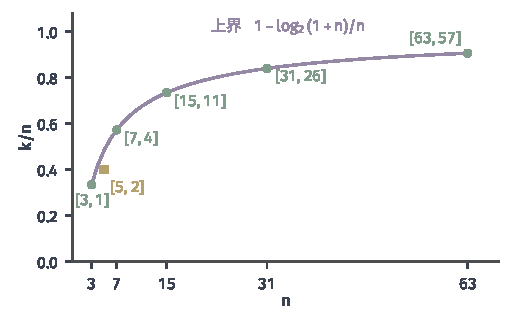
\includegraphics[width=88mm]{figures/07-probability/06-channel-coding/matplotlib/ccode-hamming-bound/figure.pdf}
 \caption{纠单错二元码的球填充界$k/n\leq1-\log_2(1+n)/n$（紫线，按整数$n$连成）。绿点是块长$n=2^{r}-1$的Hamming码，恰好落在界上；$[3,1]$即三次重复码。黄色方块是$[5,2,3]$码，位于界的下方。}
 \label{fig:ccode-hamming-bound}
\end{BookInlineFigure}

球填充界只依赖“保证纠正$t$个”这一组合要求，与信道的翻转概率无关。在$p=0.1$的信道上，块长$1000$时平均有$100$个翻转，若要求保证纠正它们，需要
\[
 R\leq1-\frac{\log_2V(1000,100)}{1000}\approx0.535 ,
\]
而且保证纠正$100$个并不够：翻转个数超过$100$的概率约为$0.47$。概率意义下的错误需要另外的论证。

\paragraph{错误概率的下界}
现在允许任意码本、任意解码器，只问块错误概率能小到什么程度。思路仍然是“领地”：解码器把每个接收块判给一条消息，于是$2^{n}$个接收块被分成$M$个判决区域$D_1,\dots,D_M$。消息$m$判对的概率是码字$\bm{c}_m$的输出落在$D_m$中的概率。一个区域能“接住”多少概率，取决于它包含哪些接收块；最划算的是包含离码字最近的那些，也就是一个Hamming球。

为了精确表述，把一条码字到全部$2^{n}$个接收块的转移概率从大到小排成
\[
 a_1\geq a_2\geq\cdots\geq a_{2^{n}} .
\]
在二元对称信道上，$W^{n}(\bm{y}\mid\bm{c})=p^{d}(1-p)^{n-d}$，其中$d=\operatorname{dist}(\bm{y},\bm{c})$；与码字相距$d$的接收块有$\binom nd$个，所以这个排列对每条码字都相同。定义
\begin{equation}
 g(s)=\sum_{i=1}^{\lfloor s\rfloor}a_i+(s-\lfloor s\rfloor)\,a_{\lfloor s\rfloor+1},\qquad 0\leq s\leq2^{n},
 \label{eq:ccode-g}
\end{equation}
约定$a_{2^{n}+1}=0$。整数$s$处，$g(s)$是最大的$s$个转移概率之和；整数之间线性插值。

\begin{theorem}[有限块长的逆向界]
\label{thm:ccode-sphere-converse}
在二元对称信道上，任意$M$条码字、块长为$n$的码，配合任意确定的解码器，均匀消息下的平均块错误概率满足
\begin{equation}
 1-P_{\mathrm{e}}\leq g\Bigl(\frac{2^{n}}{M}\Bigr) .
 \label{eq:ccode-sphere-converse}
\end{equation}
\end{theorem}

\begin{proof}
设判决区域为$D_1,\dots,D_M$，它们两两不相交，并集是全部$2^{n}$个接收块，所以
\[
 \sum_{m=1}^{M}\lvert D_m\rvert=2^{n} .
\]
均匀消息下判对的概率是
\[
 1-P_{\mathrm{e}}=\frac1M\sum_{m=1}^{M}\ \sum_{\bm{y}\in D_m}W^{n}(\bm{y}\mid\bm{c}_m) .
\]

第一步，固定$m$。$D_m$含$\lvert D_m\rvert$个接收块，它们的转移概率是$a_1,\dots,a_{2^{n}}$中的$\lvert D_m\rvert$个，和不超过最大的$\lvert D_m\rvert$个之和：
\[
 \sum_{\bm{y}\in D_m}W^{n}(\bm{y}\mid\bm{c}_m)\leq g(\lvert D_m\rvert) .
\]

第二步，$g$是凹函数。它在每个区间$[i-1,i]$上是斜率为$a_i$的线段，斜率随$i$不增，所以$g$是凹的。对有限个点取平均，凹函数满足Jensen不等式：
\[
 \frac1M\sum_{m=1}^{M}g(\lvert D_m\rvert)\leq g\Bigl(\frac1M\sum_{m=1}^{M}\lvert D_m\rvert\Bigr)=g\Bigl(\frac{2^{n}}{M}\Bigr) .
\]
两步合起来就是式~\eqref{eq:ccode-sphere-converse}。
\end{proof}

这个界的读法是：最理想的情形是每条码字恰好独占一个大小为$2^{n}/M$、由离它最近的接收块组成的区域。码字越多，每条分到的区域越小，能接住的概率越少。证明中两个不等号同时取等，要求每个判决区域都是以码字为中心的Hamming球（必要时连同一部分下一层），且大小都相同。完备码满足这一点。

对$n=7$、$M=16$，$2^{7}/16=8$，最大的$8$个转移概率是距离$0$的一个与距离$1$的七个，于是
\[
 1-P_{\mathrm{e}}\leq0.9^7+7\times0.1\times0.9^6=0.85031 .
\]
上一节算出Hamming码的块错误概率恰好是$0.14969$，等号成立。所以在$p=0.1$的二元对称信道上，没有任何$16$条码字、块长为$7$的码，配合任何解码器，能比$[7,4,3]$ Hamming码做得更好。

同样的计算也适用于重复码。块长$7$、两条码字时$2^{7}/2=64$，而半径为$3$的球恰含
\[
 V(7,3)=1+7+21+35=64
\]
个串，所以
\[
 1-P_{\mathrm{e}}\leq\mathbb{P}(\text{翻转个数}\leq3)=0.997272 .
\]
七次重复码的错误概率是$0.002728$，又一次取到等号：长度为奇数$n=2t+1$的重复码也是完备码，它的两个半径为$t$的球恰好平分全部$2^{n}$个串。于是在$p=0.1$的信道上，块长为$7$的码即使只传一个比特，错误概率也不可能低于$0.0027$，要求$10^{-3}$就必须加长块。

反过来，给定目标错误$\varepsilon$，式~\eqref{eq:ccode-sphere-converse}限制了码字个数。$g$单调增，设$s^{*}$是使$g(s)\geq1-\varepsilon$的最小$s$，则任何满足$P_{\mathrm{e}}\leq\varepsilon$的码都有$2^{n}/M\geq s^{*}$，即
\begin{equation}
 R\leq1-\frac{\log_2s^{*}}{n} .
 \label{eq:ccode-converse-rate}
\end{equation}
$s^{*}$可以按距离由近到远累加$\binom nd p^{d}(1-p)^{n-d}$精确算出。

\paragraph{随机码的保证}
另一个方向要证明某个码确实能做到。第~\ref{chap:discrete-channel-capacity}章用随机码本证明了可达性，那里的估计是为渐近目的设计的；在二元对称信道上，同样的思路可以给出一个对每个$n$都能精确计算的界，称为\term{随机编码并集界}。

\begin{theorem}[随机编码并集界]
\label{thm:ccode-rcu}
在翻转概率$p<\tfrac12$的二元对称信道上，对任意块长$n$与码字个数$M\geq1$，存在一个码本，配合最小距离译码，其平均块错误概率满足
\begin{equation}
 P_{\mathrm{e}}\leq\sum_{k=0}^{n}\binom nk p^{k}(1-p)^{n-k}\min\Bigl\{1,\ (M-1)\,\frac{V(n,k)}{2^{n}}\Bigr\} .
 \label{eq:ccode-rcu}
\end{equation}
\end{theorem}

\begin{proof}
独立地从$\{0,1\}^{n}$中均匀抽取$M$条码字。解码器选距离最近的码字，并且只要有别的码字与接收块的距离不超过正确码字，就把这次传输算作错误；这只会高估错误。

固定消息$m$，设信道翻转了$k$位，接收块为$\bm{y}$，于是$\operatorname{dist}(\bm{y},\bm{c}_m)=k$。判错要求某个$j\neq m$满足$\operatorname{dist}(\bm{c}_j,\bm{y})\leq k$。$\bm{c}_j$与$\bm{c}_m$、与信道噪声都独立，并且在$\{0,1\}^{n}$上均匀，所以对每个固定的$\bm{y}$，
\[
 \mathbb{P}\bigl(\operatorname{dist}(\bm{c}_j,\bm{y})\leq k\bigr)=\frac{V(n,k)}{2^{n}} .
\]
对$M-1$个竞争者用并集上界，再与$1$取小，得到在给定$k$时判错的条件概率不超过
\[
 \min\Bigl\{1,\ (M-1)\,\frac{V(n,k)}{2^{n}}\Bigr\} .
\]
翻转个数$k$服从$\operatorname{Bin}(n,p)$，对$k$取平均，得到对码本与噪声一起取期望后，消息$m$的错误概率不超过式~\eqref{eq:ccode-rcu}右边。这个界对每个$m$相同，所以随机码本的平均错误概率的期望也不超过它；一个随机变量不可能处处大于自己的均值，于是某个具体码本的平均错误概率不超过它。
\end{proof}

右边的$\min$体现了两种错误来源的分工。翻转少时，$V(n,k)/2^{n}$极小，竞争码字几乎不可能靠得更近；翻转多到使$(M-1)V(n,k)\geq2^{n}$时，球内平均已有一个以上的竞争者，这时直接按判错计算。这正是第~\ref{chap:discrete-channel-capacity}章典型性论证的有限块版本。

\paragraph{两条界之间}
对给定的$n$与目标错误$\varepsilon$，用二分法求出使式~\eqref{eq:ccode-rcu}右边不超过$\varepsilon$的最大$\log_2M$，就得到随机码能保证的码率；式~\eqref{eq:ccode-converse-rate}给出任何码都不能超过的码率。真正最优的码率夹在两者之间。图~\ref{fig:ccode-finite-rate}在$p=0.1$、$\varepsilon=10^{-3}$下画出这两条曲线。

\begin{BookInlineFigure}
 \centering
 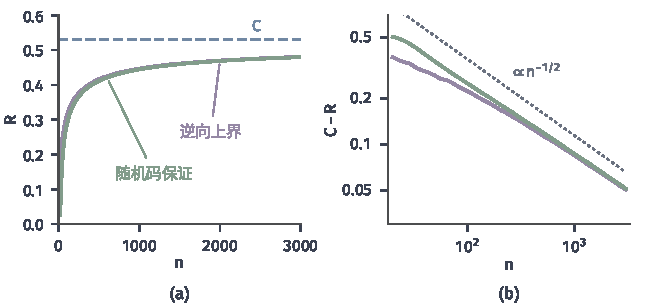
\includegraphics[width=110mm]{figures/07-probability/06-channel-coding/matplotlib/ccode-finite-rate/figure.pdf}
 \caption{$p=0.1$的二元对称信道上，平均块错误概率不超过$10^{-3}$时的码率界限，均为精确计算。紫线为式~\eqref{eq:ccode-converse-rate}的逆向上界，任何码都在它下方；绿线为由式~\eqref{eq:ccode-rcu}得到的随机码保证，存在码达到它；蓝色虚线为容量$C=0.531$。(a) 码率随块长$n$的变化，两条曲线几乎重合；(b) 两者与容量的差$C-R$，双对数坐标，灰色点线是斜率$-\tfrac12$的参照。}
 \label{fig:ccode-finite-rate}
\end{BookInlineFigure}

从图中读出几组数：$n=100$时，最优码率在$0.281$与$0.309$之间；$n=1000$时，在$0.444$与$0.447$之间。容量是$0.531$，所以开头的问题有了确定的答案：块长$1000$、错误不超过$10^{-3}$，码率至多约$0.447$，比容量低约$16\%$；也就是说，冗余至少要占$55\%$，而容量只要求约$47\%$。图(b)显示，两条界与容量之差都大致按$n^{-1/2}$缩小。这是对这两条界的数值观察，直观上来自翻转个数$\operatorname{Bin}(n,p)$的波动：它的标准差是$\sqrt{np(1-p)}$，为了以$1-\varepsilon$的概率覆盖这些波动，每个码字的领地要比“平均翻转个数”多留出与$\sqrt n$同阶的余量，摊到每个符号上就是$n^{-1/2}$。把这一直观变成关于最优码率的定理，需要对中心极限定理的误差作定量控制，本章不作证明。

\paragraph{计算的代价}
两条界都只关心错误概率，没有计入编码与译码的成本。随机码保证的码在$n=1000$、$R=0.444$时有$2^{444}$条码字，既无法存储，也无法逐一比较。即使改用线性码，综合征对照表也有$2^{556}$项。下面的表把本章出现的几种做法放在一起。

\begin{BookInlineTable}
 \centering
 \caption{有限块编码的码率、错误与计算代价（二元对称信道，$p=0.1$）}
 \label{tab:ccode-cost}
 \begin{tabular}{lllll}
 \toprule
 方案 & 码率 & 块错误 & 存储 & 每块译码运算 \\
 \midrule
 三次重复 & $1/3$ & $0.028$ & 无 & $3$次 \\
 $[5,2,3]$线性码 & $0.4$ & $0.067$ & $8$项表 & $15$次 \\
 $[7,4,3]$ Hamming & $4/7$ & $0.150$ & 无 & $21$次 \\
 $[n,k]$线性码 & $k/n$ & 依码而定 & $2^{n-k}$项表 & $(n-k)n$次 \\
 随机码本 & $\log_2M/n$ & 式~\eqref{eq:ccode-rcu} & $Mn$比特 & $Mn$次 \\
 \bottomrule
 \end{tabular}
\end{BookInlineTable}

表中的“每块译码运算”只计多数判决、综合征或逐一比较所需的比特运算，不计查表与读写；$[n,k]$线性码一行假设对照表已经存在，建表本身要枚举错误向量。块错误概率一列中，重复码和$[5,2,3]$码针对的消息比特数不同，比较时要换算到相同的消息长度，如第~\ref{sec:ccode-syndrome}小节所做。

\paragraph{三类陈述}
本节的结论可以归为三类，它们回答不同的问题。
\begin{itemize}
 \item 理论下界：球填充界与逆向界~\eqref{eq:ccode-sphere-converse}对所有码、所有解码器成立，说明“不可能更好”，但不提供任何码。
 \item 构造保证：随机编码并集界说明“存在至少这样好的码”，同时只给出一个需要指数级存储与搜索的码，不说明怎样找到便宜的码。
 \item 实际计算：重复码、$[5,2,3]$码与Hamming码的错误概率是对具体码和具体译码器的精确计算，它们落在界的哪一侧、离界多远，才说明这个构造好不好。
\end{itemize}
容量是这几类陈述在块长趋于无穷时的共同极限。它约束了渐近可达的速率，单凭它不能回答给定块长需要多少冗余，也不能回答需要多大的计算量。
